\chapter{详细设计与实现}
\vspace{7pt}

在系统总体设计的基础上，本章进一步给出各核心模块的详细实现方案。首先阐述RAG文档解析模块中PDF扫描件与文本件的双模式解析逻辑，以及文本分块与向量索引的构建过程；随后介绍多智能体协作建模引擎中用例图、类图与时序图Agent的具体实现，重点说明防止孤立角色的约束优化、Prompt工程及断点机制的落地方式；接着论述基于Jinja2的模板渲染与代码清洗优化；最后展示前端可视化平台中Monaco Editor双向同步与一键打包导出功能的实现细节。上述实现共同构成了完整的自动化用例建模系统。

\section{RAG文档解析模块实现}

\subsection{PDF扫描件与文本件解析逻辑}

文档解析模块是自动化用例建模系统的入口，负责将用户上传的需求文档转换为可供大语言模型处理的纯文本内容。实际工程中的需求文档格式多样，既包含可直接提取文字的文本型PDF，也有经扫描生成的图片型PDF，还有纯文本格式的需求描述，系统需要对这些不同类型提供兼容处理能力。

系统采用双模式解析策略，根据文档的实际内容特征自动选择处理路径。对于文本型PDF，系统调用pdfplumber库进行页面级文本提取。pdfplumber逐页解析PDF内部文字层的数据，提取过程中保留原始的段落边界和页面分隔信息，提取后的文本按页标记进行分段，以便后续分块和检索时保留文档的结构信息。实现中，\texttt{\_parse\_pdf}函数将文件内容封装为字节流，遍历PDF的每一页并调用\texttt{extract\_text}方法，当某页无可提取文字时返回空字符串，最终将所有页面文本拼接为完整的文档字符串。

对于扫描件PDF，由于文件中缺少文字层信息，pdfplumber提取的文本长度通常极短。系统据此设计了扫描件自动检测机制：当一次PDF解析获得的文本总字符数低于预设阈值时，即判定该文档为扫描件，触发基于多模态视觉模型的识别流程。该流程首先利用PyMuPDF将PDF的每一页渲染为PNG格式的图片，生成的图片数据以字节数组形式暂存于内存，随后逐一上传至对象存储服务并获取签名URL。为避免单次调用视觉模型时图片数量过多导致Token溢出，系统将图片列表分批调用Qwen-VL-Plus模型，模型接收图片内容并输出从中识别出的文字描述，最后将所有批次的识别结果合并为完整的文档文本。

文档解析完成后，系统根据文本长度和文档类型判断项目复杂度。当解析出的文本长度超过一千字符或文档类型为PDF时，项目被标记为复杂项目。对于复杂项目，系统自动触发智能模块拆解流程，由大语言模型对完整需求文本进行结构性分析，将其划分为若干粒度适中的功能子模块，每个模块拥有独立的核心需求文本和独立的LangGraph工作流会话标识。用户确认或调整模块划分后，各模块即作为独立的建模单元进入后续处理流程。模块拆分页面如图5.1所示。

% 图5.1 模块拆分页面
\begin{figure}[htbp]
    \centering
    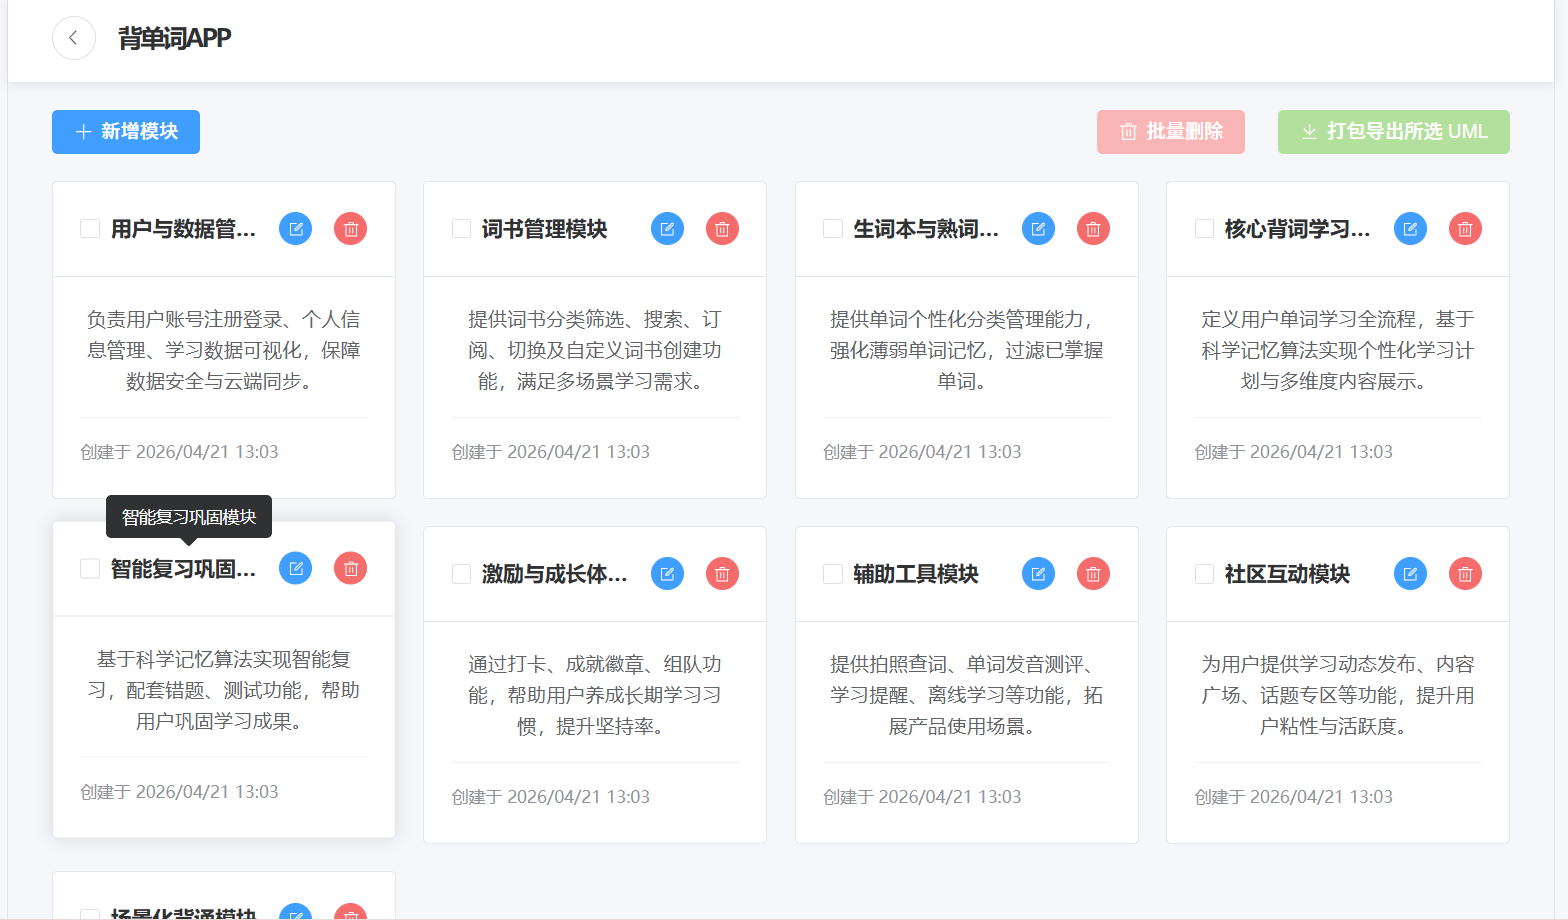
\includegraphics[width=160mm]{docs/imgs/模块拆分页面.png}
    \caption{模块拆分页面}
    \label{fig:module_splitting}
\end{figure}

\subsection{文本分块与向量索引构建}

在模块拆解完成后，系统立即基于完整的原始需求文档构建检索增强生成所需的向量索引。文本分块采用基于句子边界的切分策略，以中文标点符号句号、感叹号、问号、分号以及换行符作为切分触发符。当遇到这些分隔符且当前累积长度达到设定阈值时，即将累积内容作为一个独立的文本块输出。对于未达到分隔符但长度超限的文本，系统引入jieba分词工具进行二次切分，按累积长度重新组装为符合尺寸要求的文本块。

文本分块完成后，系统调用paraphrase-multilingual-MiniLM-L12-v2嵌入模型将每个文本块转化为固定维度的稠密向量。生成的向量连同文本块内容和元数据通过ChromaDB的add接口批量写入以项目为单位的向量集合中。在存储之前，系统会先清除该项目的旧集合，确保每次索引都基于最新的文档内容。

在后续的建模阶段，当用户对任一子模块启动用例图、类图或时序图生成时，系统以该子模块的需求描述作为查询条件，通过同一嵌入模型将其向量化后向ChromaDB发起语义检索请求，获取与其语义最相关的原文段落。检索结果被格式化为带有段序号的上下文文本，拼接到发送给大语言模型的提示词中。通过这种“全局索引、按需检索”的架构，每个模块的建模过程能够获得跨越模块边界的上下文信息，保证了参与者和用例在整个系统范围内的一致性，有效避免了因模块拆分而导致的信息碎片化。

\section{多智能体协作建模引擎实现}

\subsection{用例图Agent实现：防止孤立角色的约束优化}

用例图生成过程的首要任务是提取系统参与者与用例。大语言模型在处理此任务时，有时会将内部组件或被动实体错误地识别为参与者，例如将数据库、后台服务或算法模块当作Actor。此外，模型还可能生成“系统”这样没有实际关联用例的孤立参与者，这在UML规范中是应当避免的情况。

针对上述问题，系统在用例提取的提示词模板（ee\_template）中嵌入了严格的约束规则。规则明确指出，参与者必须是系统外部的人、第三方系统或硬件设备，不允许将数据库、后台服务器、算法模块等内部组件列为参与者。规则进一步强调禁止孤立参与者，要求提取出的每一个参与者必须至少关联一个用例，如果某个实体仅仅是背景存在而没有具体的交互动作，则不应将其提取为Actor。这些约束规则以负面示例和正面示例相结合的方式编写在提示词中，使模型在进行实体识别时具备更强的边界判断能力。

在Agent实现层面，extract\_entities\_node函数在调用大语言模型前首先检查状态池中是否已存在用户确认的参与者和用例列表。若confirmed\_actors或confirmed\_usecases字段非空，说明用户已经对提取结果进行了人工审核和修改，此时函数将直接返回确认后的列表，不再调用大语言模型进行新的提取。这一锁定机制确保了用户的修正不会被后续自动化流程覆盖。若确认列表为空，函数则使用上述带有约束的提示词模板构造请求，调用openai\_chat\_completion接口，并以JSON模式要求模型返回结构化数据。返回的JSON被解析为参与者列表、用例列表以及角色到用例的映射字典。这一设计在发挥大语言模型自动化提取能力的同时，通过人工确认节点和锁定机制保证了结果的可控性。

\subsection{类图与时序图Agent实现：Prompt工程}

类图生成包含三个顺序执行的Agent节点，分别负责实体类的识别、类属性与方法的提取以及类间关系的推理。每个Agent节点的提示词模板都经过针对性设计，以引导模型产生符合期望的结构化输出。

类实体提取提示词（cd\_entity\_prompt）要求模型从需求文本中读出系统的核心域对象，将其作为类图的实体类。提示词明确指示模型仅输出提供的classes列表中的类，不允许创建新类。这一限定与锁定机制配合，防止模型在后续步骤中自行添加未经用户确认的类名。

类属性方法提取提示词（cd\_attr\_method\_prompt）对属性和方法给出了明确界定：属性是描述类所拥有的特征或状态数据的名词，如用户的“用户名”和“密码”；方法是描述类所执行的操作或行为的动词，如“登录()”和“创建订单()”。提示词特别强调必须仅为已确认的classes列表中的类提取属性和方法，严禁创建列表中不存在的类，从而使属性方法的提取严格限制在已确认的类范围之内，避免了数据污染。

时序图参与者提取提示词（sd\_participant\_prompt）要求模型按照UML规范将参与者分为五类：actor表示外部用户或角色，boundary表示界面或边界对象，control表示控制对象，entity表示实体对象，database表示数据库。提示词同时限制模型只能从已确认的角色列表和类列表中选取参与者，防止引入未定义的实体。

在代码实现中，每个Agent节点均采用统一的结构：首先检查锁定状态和确认列表，根据需要过滤待处理的实体集合；然后通过get\_template函数加载对应的提示词模板，填充当前的需求文本和实体数据；随后根据任务复杂度选择推理模型或对话模型进行调用；最后使用parse\_json\_from\_response工具函数从容错处理后的响应中提取JSON数据，更新状态池。这种模板化的Prompt工程方法使得每个Agent的语义目标清晰聚焦，有效提升了各子任务的执行精度。张戈等人\cite{zhang2026teaching}在UML建模的智能化实践研究中也验证了类似结论，即通过设计具体的任务指令与示范性数据，能够有效引导大语言模型更精准地完成从自然语言业务描述到UML图的转换。

\subsection{断点机制在Agent节点中的具体实现}

断点机制是LangGraph提供的人机交互基础设施。系统在构建工作流图时，通过compile函数的interrupt\_before参数指定两个断点位置：第一个位于relationship\_agent节点之前，第二个位于class\_attr\_method\_agent节点之前。interrupt\_before接受一个节点名称列表，当工作流执行到这些节点时，LangGraph会自动挂起执行并保存当前状态快照。

断点挂起后，系统的前端界面从API获取当前的中间态JSON数据，将其渲染为可编辑的表格。用户可以在表格中对提取出的角色、用例或类名列表进行修改确认。确认操作触发的API请求将用户编辑后的数据以confirmed\_data形式发送至后端。在resume\_and\_generate方法中，系统首先通过app\_graph.get\_state获取断点处的完整状态，然后将用户提交的确认数据与当前状态合并。合并后，系统根据确认数据中的字段设置相应的锁定标志：若confirmed\_data中包含classes，则设置confirmed\_classes；若包含actors，则设置confirmed\_actors；若包含usecases，则设置confirmed\_usecases。这些锁定标志在后续Agent节点中被检查，用以强制Agent只能处理已确认的实体，不得新增。

状态更新完成后，系统调用app\_graph.ainvoke并传入None作为输入，通知LangGraph从当前状态继续执行工作流。LangGraph内部从断点节点开始执行，后续节点按照图的有向边依次被激活，直至到达终止节点。这一机制以极低的工程代价实现了复杂工作流中的人工介入，使用户对自动化建模过程拥有最终的决策权。用例图确认表格和类图确认表格分别如图5.2和图5.3所示。

% 图5.2 用例图确认表格
\begin{figure}[htbp]
    \centering
    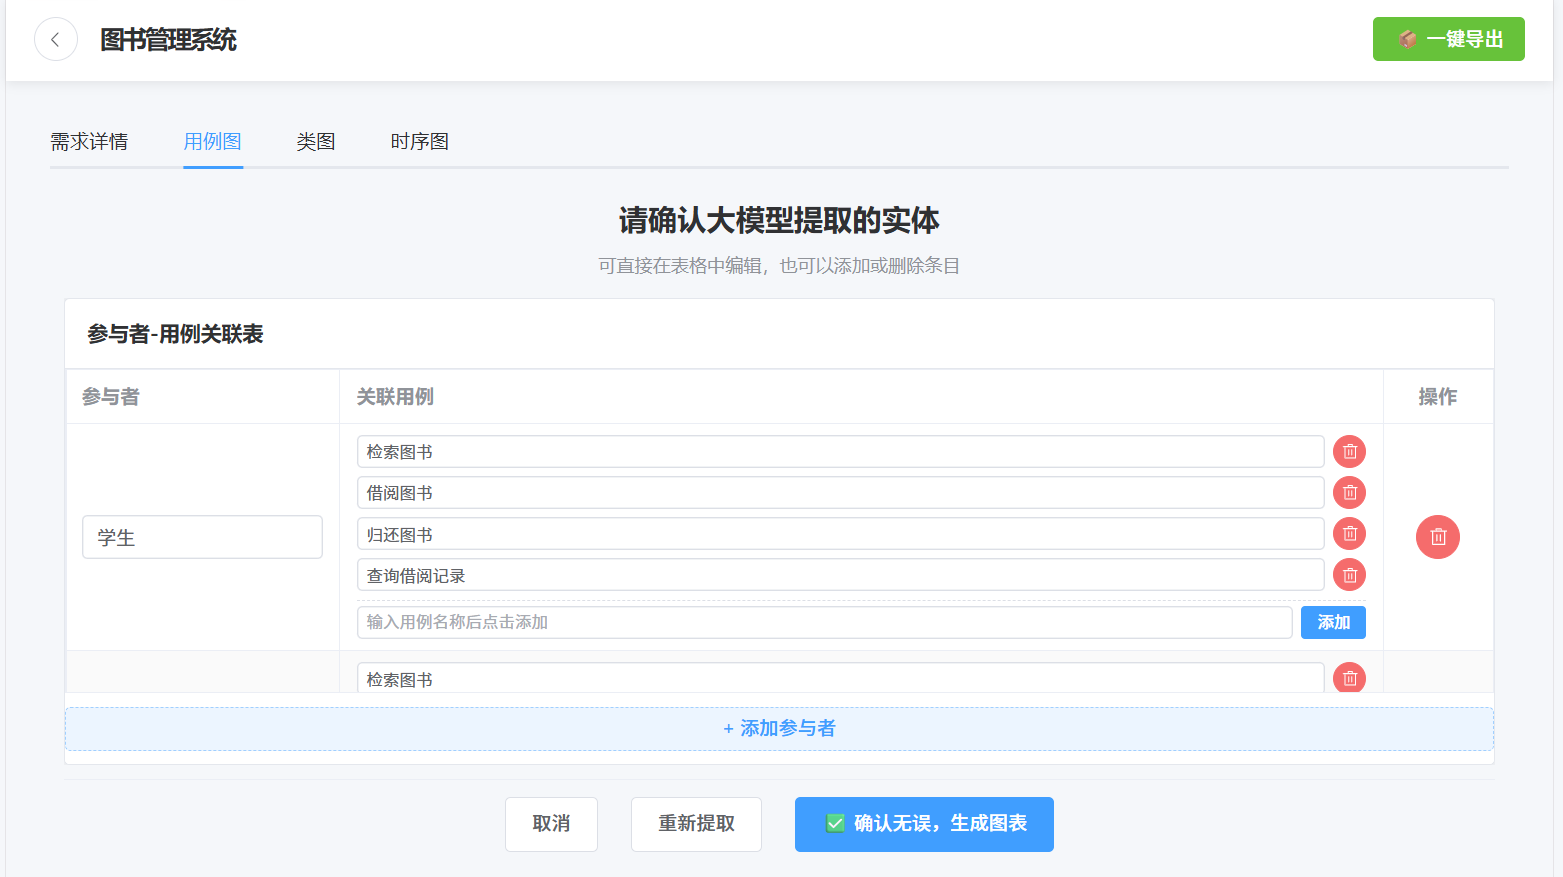
\includegraphics[width=160mm]{docs/imgs/用例图确认表格.png}
    \caption{用例图确认表格}
    \label{fig:use_case_table}
\end{figure}

% 图5.3 类图确认表格
\begin{figure}[htbp]
    \centering
    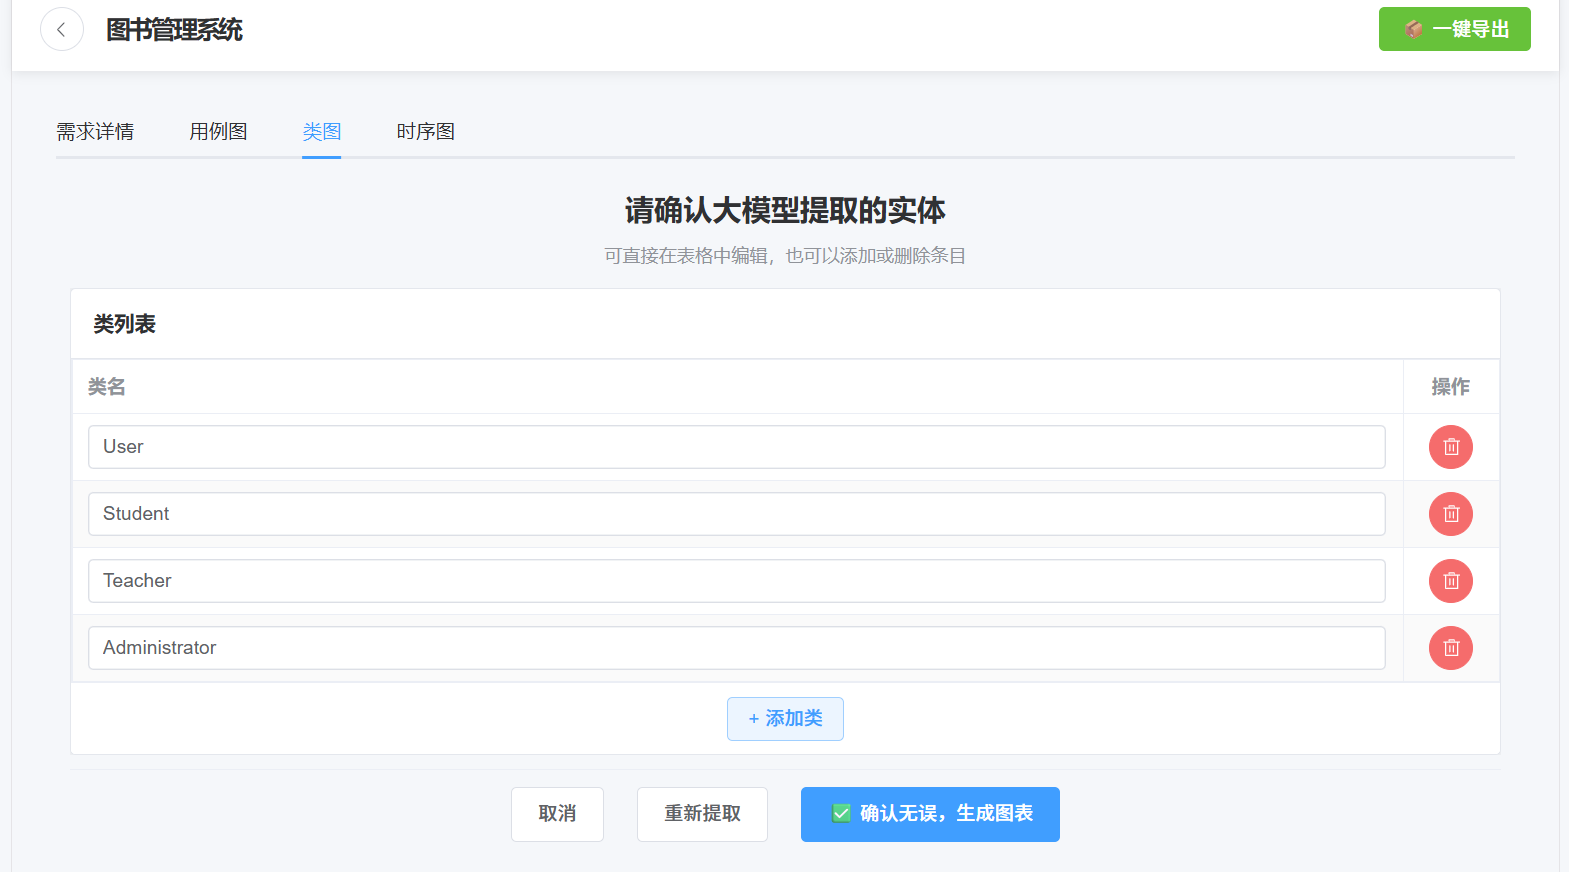
\includegraphics[width=160mm]{docs/imgs/类图确认表格.png}
    \caption{类图确认表格}
    \label{fig:class_table}
\end{figure}

\section{自动化渲染与模板引擎优化}

\subsection{基于Jinja2的PUML动态模板组装}

PlantUML代码的生成采用Jinja2模板引擎实现数据与表示的分离。针对用例图、类图和时序图，系统分别设计了独立的Jinja2模板文件。模板内部使用Jinja2的控制结构（如for循环和if条件）动态遍历建模数据，生成符合PlantUML语法规范的文本代码。

渲染服务通过\texttt{\_render\_and\_save}等函数实现对模板的加载、数据渲染和PlantUML图片生成。函数内部首先创建Jinja2环境并指定模板目录，然后通过get\_template加载对应图表类型的模板文件，将传入的数据上下文字典作为参数调用render方法，生成最终的PUML代码。生成后的代码一方面保存为文本文件供用户下载，另一方面通过PlantUML官方服务器渲染为PNG图片并保存，或直接生成编码后的在线URL返回给前端展示。

\subsection{工程优化：代码清洗}

在实际运行中，大语言模型生成的PlantUML代码可能包含一些导致渲染失败的瑕疵。常见的问题包括：代码中存在多余的空白行、在JSON输出中被包裹了Markdown代码块标记、时序图文件名中包含文件系统不接受的非法字符，以及关系定义中引用了已被用户删除的实体名称等。为确保PlantUML渲染引擎能够成功解析每一次生成的代码，系统在多个环节植入了代码清洗逻辑。

代码清洗的第一个环节是JSON提取容错。大语言模型在输出JSON时，有时会在JSON前后附加说明文字，或将JSON包裹在Markdown代码块中。extract\_json\_from\_response工具函数专门处理此类情况。该函数首先检测响应文本中是否存在“\textasciigrave\textasciigrave\textasciigrave json ... \textasciigrave\textasciigrave\textasciigrave”模式，若存在则提取代码块内的内容。若未匹配到代码块，则尝试在全文寻找最外层的大括号或中括号对，作为JSON候选字符串。在parse\_json\_from\_response函数中，还会对多个候选字符串进行逐个解析尝试，选取第一个可成功解析为JSON对象的字符串作为最终结果。这种层层容错的设计显著提升了对模型非标准输出的适应能力。

第二个清洗环节是空白行与非法字符的处理。在最终的PUML代码生成路径中，各Agent的输出在写入状态池前已经过strip处理去除首尾空白。在时序图文件名的生成过程中，系统调用字符串替换方法去除用例名称中的“/”和“\textbackslash”字符，因为这些字符在文件系统中属于路径分隔符，直接作为文件名会导致保存失败。

第三个清洗环节是逻辑约束校验。在用例图的关系分析Agent中，解析出的关系数据在写入状态池前会经过过滤：仅保留那些涉及已确认参与者和用例的关系记录。这样确保了即使用户在前端删除了某些实体，图中也不会出现悬挂的连线引用。这些清洗措施共同保证系统输出代码的渲染成功率趋近于百分之百。

\section{可视化前端平台实现}

\subsection{Monaco Editor双向同步机制实现}

前端工作区的核心可视化编辑组件为Monaco Editor，通过@guolao/vue-monaco-editor包集成到Vue 3项目中，如图5.4所示。组件的配置选项中，language设为plaintext以支持PlantUML语法的基本高亮，theme选用vs-dark深色主题以提升代码可读性，wordWrap开启自动换行以适应长行内容，automaticLayout开启自适应布局使编辑器随容器尺寸变化而自动调整。

% 图5.4 PlantUML代码编辑区
\begin{figure}[htbp]
    \centering
    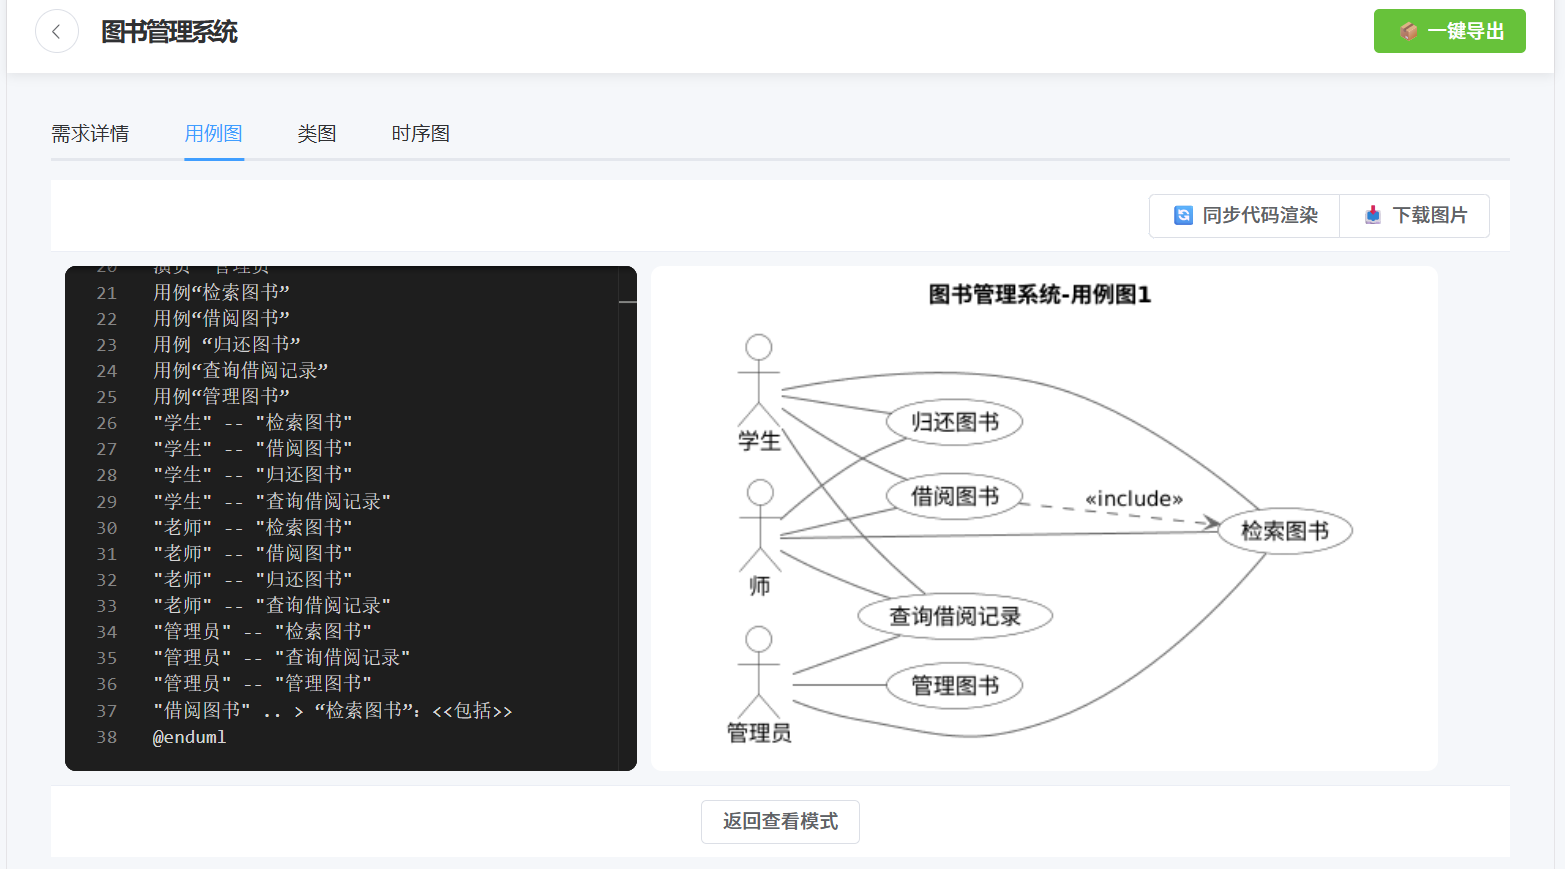
\includegraphics[width=160mm]{docs/imgs/PlantUML代码编辑区.png}
    \caption{PlantUML代码编辑区}
    \label{fig:code_editor}
\end{figure}

双向同步机制连接了表格视图与代码视图。表格视图是用户确认数据的主要界面，展示提取出的参与者、用例、类名等结构化信息。当用户在表格中修改数据并触发“生成”操作时，前端调用generate接口，将当前表格数据作为confirmed\_data发送至后端。后端恢复工作流执行并渲染生成新的PlantUML代码后，返回代码字符串和图片URL。前端接收到响应后，使用响应式绑定将新的PUML代码赋值给编辑器绑定的变量，从而自动更新编辑器内容。同时，图片URL更新触发预览区重新加载图表渲染结果。

逆向同步的方向由编辑器到表格。当用户直接在Monaco Editor中修改PlantUML代码后，点击“同步代码渲染”按钮触发逆向同步。前端调用sync接口，将当前编辑器中的PUML代码发送至后端。后端调用PUML解析器（优先使用正则快速解析，失败时降级调用大语言模型分析），从代码中逆向提取出参与者、用例、关系等结构化数据，并重新渲染图片。前端接收到新的结构化数据后，将其更新到表格组件中，同时更新图片预览。这种双向同步使用户能够在表格引导式和代码直接编辑式两种交互模式间自由切换，满足了不同操作偏好的用户需求。

\subsection{建模资产的一键打包导出逻辑}

为方便用户将生成的UML图表应用于文档或分享，前端提供了打包导出功能，其逻辑示意如图5.5所示。该功能基于jszip和file-saver两个JavaScript库实现。jszip用于在浏览器端创建和操作ZIP压缩包，file-saver用于触发浏览器的文件下载行为。

导出逻辑封装在工具函数中。系统首先通过获取项目资产列表接口拿到当前项目下所有已确认的UML图表信息，包括用例图、类图和多个时序图的图片URL。打包函数为每种图表在ZIP中创建相应的文件夹结构：用例图和类图图片以中文名称命名，时序图图片以“用例名称-时序图.png”格式命名。函数逐一fetch这些图片URL，将获取到的blob数据通过jszip的file方法添加到ZIP实例中。所有文件添加完毕后，调用generateAsync方法生成ZIP压缩包的blob对象，最后通过file-saver的saveAs方法触发浏览器下载，文件名以项目名称命名。整个打包过程在浏览器端完成，无需服务器参与，既减轻了服务端压力，也保证了数据隐私。

% 图5.5 建模资产的一键打包导出
\begin{figure}[htbp]
    \centering
    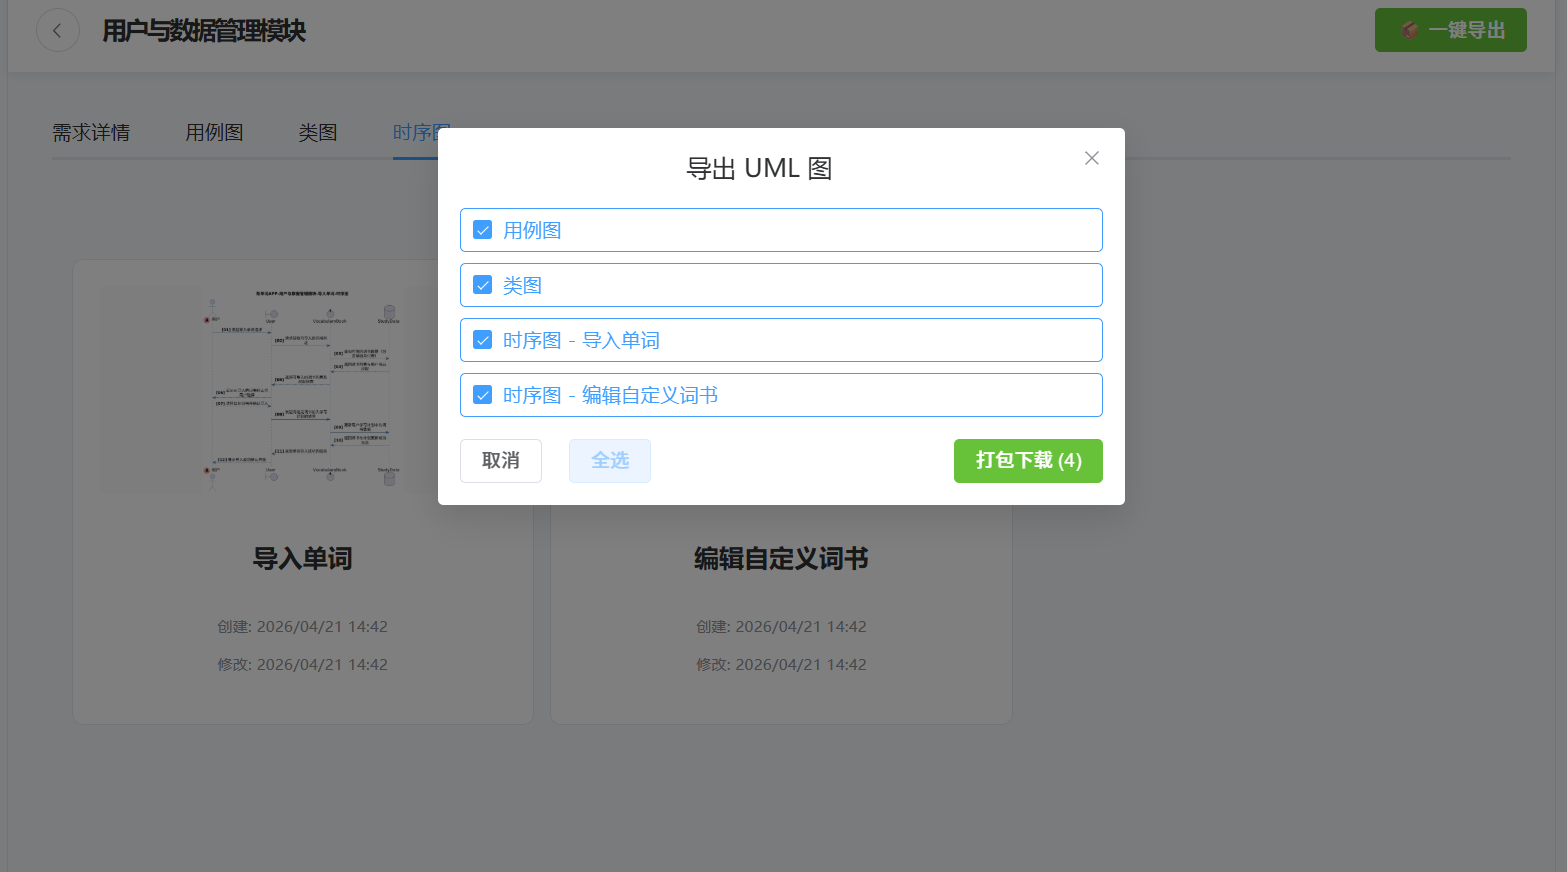
\includegraphics[width=160mm]{docs/imgs/建模资产的一键打包导出.png}
    \caption{建模资产的一键打包导出}
    \label{fig:export_logic}
\end{figure}

\section{本章小结}
本章详细阐述了自动化用例建模系统的核心模块实现。在RAG文档解析方面，实现了PDF文本件与扫描件的双模式解析，并构建了基于句子边界的文本分块与ChromaDB向量索引。多智能体协作建模引擎中，通过约束优化和Prompt工程分别实现了用例图、类图与时序图的Agent，并基于LangGraph断点机制完成了人机协同的确认流程。模板渲染层面，采用Jinja2动态组装PUML代码，并结合JSON容错、字符清洗与逻辑校验等工程优化提升了渲染成功率。前端可视化平台则实现了Monaco Editor与表格的双向同步，以及建模资产的一键打包导出。上述实现为下一章的系统实验评测与结果分析提供了完整的可运行系统基础。